\section{Quadcopter dynamics}

To understand how the low-level controller takes a velocity vector as input
and computes the desired rotor speed for each propeller, the quadrotor dynamic
model must be described.
Fig.~\ref{fig:aero-dynamics} illustrates the Intel Aero drone configuration
with its reference frames. The global fixed frame is $\mathcal{F}_W =
\{\vec{\mathbf{x}}_W, \vec{\mathbf{y}}_W, \vec{\mathbf{z}}_W\}$ and the body
frame is $\mathcal{F}_B = \{\vec{\mathbf{x}}_B, \vec{\mathbf{y}}_B,
\vec{\mathbf{z}}_B\}$. Assuming an UAV is a rigid body, the origin of
$\mathcal{F}_B$ is located at its center of gravity. 

\begin{figure}[h!]
  \centering
  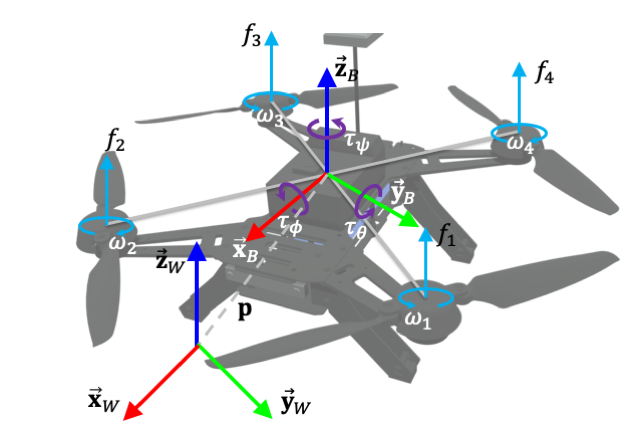
\includegraphics[width=\textwidth]{figure/aero_dynamics.png}
  \caption{Model of Intel Aero's quadrotor dynamics.}
  \label{fig:aero-dynamics}
\end{figure}

In a Cartesian coordinate system, the position of the UAV is given by 
$\mathbf{p} = \begin{bmatrix} x & y & z \end{bmatrix}^T \in \mathbb{R}^3$,
and the attitude by the Euler angles
$\mathbf{o} = \begin{bmatrix} \phi & \theta & \psi\end{bmatrix}^T \in
\mathbb{R}^3$.
The time derivative of the position gives the velocity
$\mathbf{v} = \begin{bmatrix}\dot{x} & \dot{y} & \dot{z}\end{bmatrix}^T =
\begin{bmatrix} u & v & w \end{bmatrix}^T \in \mathbb{R}^3$
of the quadcopter in 
$\mathcal{F}_W$, while $\mathbf{v}_B \in \mathbb{R}^3$
is its velocity in $\mathcal{F}_B$. The relation between
$\mathbf{v}$ and $\mathbf{v}_B$ is given by

%%%%%%%%%%%%%%%%%
\begin{equation}
  \mathbf{v} = \mathbf{R} \mathbf{v}_B,
  \label{eq:linear_velocity}
\end{equation}
%%%%%%%%%%%%%%%%%

in which $\mathbf{R} \in \mathsf{SO}(3)$ is the rotation matrix from
$\mathcal{F}_B$ to $\mathcal{F}_W$:

%%%%%%%%%%%%%%%%%
\begin{equation}
  \mathbf{R} = \begin{bmatrix}c_{\psi} c_{\theta} & c_{\psi} s_{\phi}
  s_{\theta} - c_{\phi} s_{\psi} & s_{\phi} s_{\psi} + c_{\phi} c_{\psi}
  s_{\theta} \\ c_{\theta} s_{\psi} & c_{\phi} c_{\psi} + s_{\phi} s_{\psi}
  s_{\theta} & c_{\phi} s_{\psi} s_{\theta} - c_{\psi} s_{\phi} \\ -s_{\theta} &
  c_{\theta} s_{\phi} & c_{\phi} c_{\theta}\end{bmatrix},
  \label{eq:rotation_matrix}
\end{equation}
%%%%%%%%%%%%%%%%%

where $c_{\star}$ and $s_{\star}$ are $\cos\star$ and $\sin\star$,
respectively. The angular velocities are obtained from the time derivative
of the attitude $\boldsymbol{\omega} = \begin{bmatrix}\dot{\phi} &
\dot{\theta} & \dot{\psi}\end{bmatrix}^T \in \mathbb{R}^3$ in
$\mathcal{F}_W$ and $\boldsymbol{\omega}_B = \begin{bmatrix} p & q & r
\end{bmatrix}^{T} \in \mathbb{R}^3$ in $\mathcal{F}_B$, with the
following relation:

%%%%%%%%%%%%%%%%%
\begin{equation}
  \boldsymbol{\omega} = \mathbf{T} \boldsymbol{\omega}_B,
  \label{eq:angular_velocity_transformation}
\end{equation}
%%%%%%%%%%%%%%%%%

in which $\mathbf{T}$ is the coordinate transformation matrix:

%%%%%%%%%%%%%%%%%
\begin{equation}
  \mathbf{T} = \begin{bmatrix} 1 & s_{\phi} t_{\theta} & c_{\phi} t_{\theta} \\ 0
  & c_{\phi} & -s_{\phi} \\ 0 & \frac{s_{\phi}}{c_{\theta}} &
  \frac{c_{\phi}}{c_{\theta}} \end{bmatrix},
\end{equation}
%%%%%%%%%%%%%%%%%

where $t_{\star}$ denotes $\tan\star$.

The rigid body dynamic equations are derived using the Newton-Euler formulation in the body
frame:

%%%%%%%%%%%%%%%%%
\begin{equation}
  \begin{cases}
    m \dot{\mathbf{v}} = \mathbf{F} \\
    \mathbf{I} \dot{\boldsymbol{\omega}}_B = -\boldsymbol{\omega}_B \times
    \mathbf{I} \boldsymbol{\omega}_B + \boldsymbol{\tau}
  \end{cases},
  \label{eq:dynamic_equations}
\end{equation}
%%%%%%%%%%%%%%%%%

where $m$ is the mass of the UAV, $\mathbf{I} = \mathrm{diag}(I_x, I_y, I_z)$ is
the matrix of moments of inertia, $\boldsymbol{\tau} = \begin{bmatrix}
\tau_{\phi} & \tau_{\theta} & \tau_{\psi} \end{bmatrix}^T$ is the torque vector and
$\mathbf{F}$ is the force vector~\cite{Mellinger2011ICRA}:

%%%%%%%%%%%%%%%%%
\begin{equation}
  \mathbf{F} = \begin{bmatrix} -\left( c_{\phi} s_{\theta} c_{\psi} + s_{\phi}
    s_{\psi} \right) T \\ -\left( c_{\phi} s_{\theta} s_{\psi} - s_{\phi} c_{\psi}
    \right) T \\ -c_{\phi} c_{\theta} T + mg\end{bmatrix},
  \label{eq:forces}
\end{equation}
%%%%%%%%%%%%%%%%%

where $g$ is the gravitational force. Finally, from the dynamic and kinematic
equations (\ref{eq:linear_velocity}),
(\ref{eq:angular_velocity_transformation}) and (\ref{eq:dynamic_equations}),
the quadcopter model is derived~\cite{Sarabakha2016CDC}:

%%%%%%%%%%%%%%%%%
\begin{equation}
  \begin{cases}
    \dot{x} = u & \dot{u} = -\frac{c_{\phi} c_{\psi} s_{\theta} + s_{\phi} s_{\psi}}{m} T \\
    \dot{y} = v & \dot{v} = -\frac{c_{\phi} s_{\psi} s_{\theta} - c_{\psi} s_{\phi}}{m} T \\
    \dot{z} = w & \dot{w} = -\frac{c_{\phi} c_{\theta}}{m} T + g \\
    \dot{\phi} = p + s_{\phi} t_{\theta} q + c_{\phi} t_{\theta} r & \dot{p} =
    \frac{I_y - I_z}{I_x} q r + \frac{1}{I_x} \tau_{\phi} \\
    \dot{\theta} = c_{\phi} q - s_{\phi} r & \dot{p} =  \frac{I_z - I_x}{I_y} p
    r + \frac{1}{I_y} \tau_{\phi} \\
    \dot{\psi} = \frac{s_{\phi}}{c_{\theta}} p + \frac{c_{\phi}}{c_{\theta}} r
                                           & \dot{r} =  \frac{I_x - I_y}{I_z} q
                                           r + \frac{1}{I_z} \tau_{\psi}
  \end{cases},
  \label{eq:model}
\end{equation}
%%%%%%%%%%%%%%%%%

Quadcopters have four rotors: two of them forming a diagonal and rotating
clockwise, and the remaining two rotating counter-clockwise. The four rotors
generate four forces ($f_1$, $f_2$, $f_3$, $f_4$), directed along
$\vec{\mathbf{z}}_B$, and four torques ($\tau_1$, $\tau_2$, $\tau_3$,
$\tau_4$):

%%%%%%%%%%%%%%%%
\begin{equation}
  \begin{cases}
    f_i &= b \Omega_i^2 \\
    \tau_i &= dl \Omega_i^2
  \end{cases}
    , \quad i = 1,\ldots, 4,
  \label{eq:motors}
\end{equation}
%%%%%%%%%%%%%%%%

where $b$ and $d$ are force and torque coefficients of the propellers,
respectively, $l$ is the arm length from the center of gravity to each rotor,
and $\Omega_i$ is the angular velocity of the $i^{th}$ propeller.

The vector of virtual control inputs is given by~\cite{Mahony2012RAM}:

%%%%%%%%%%%%%%%%%
\begin{equation}
  \mathbf{u} = \begin{bmatrix}T & \tau_{\phi} & \tau_{\theta} & \tau_{\psi} \end{bmatrix}^T,
  \label{eq:inputs}
\end{equation}
%%%%%%%%%%%%%%%%%

in which $T$ is the total thrust along $\vec{\mathbf{z}}_B$:

%%%%%%%%%%%%%%%%%
\begin{equation}
  T = f_1 + f_2 + f_3 + f_4,
  \label{eq:T}
\end{equation}
%%%%%%%%%%%%%%%%%

while $\tau_{\phi}$, $\tau_{\theta}$ and $\tau_{\psi}$ are three rotational torques acting
around $\vec{\mathbf{x}}_B$, $\vec{\mathbf{y}}_B$ and $\vec{\mathbf{z}}_B$
axes, respectively:

%%%%%%%%%%%%%%%%%
\begin{equation}
  \begin{cases}
    \tau_{\phi} &= l (-f_2 + f_4) \\
    \tau_{\theta} &= l (f_1 - f_3) \\
    \tau_{\psi} &= -\tau_1 + \tau_2 - \tau_3 + \tau_4,
  \end{cases},
  \label{eq:tau}
\end{equation}
%%%%%%%%%%%%%%%%%

\noindent where $l$ is the arm length. By applying (\ref{eq:motors}) to
(\ref{eq:T}) and (\ref{eq:tau}), the relation between control inputs and motor
speeds is obtained, and is always invertible when $l \neq 0$, $b \neq 0$ and
$d \neq 0$. It is defined as

\begin{equation}
  \begin{cases}
    \tau_{\phi} &= l (-b\Omega_2^2 + b\Omega_4^2) \\
    \tau_{\theta} &= l (b\Omega_1^2 - b\Omega_3^2) \\
    \tau_{\psi} &= -d\Omega_1^2 + d\Omega_2^2 - d\Omega_3^2 + d\Omega_4^2,
  \end{cases},
  \label{eq:tau}
\end{equation}

or under the matrix form:
\begin{equation}
  \begin{bmatrix}
    T \\
    \tau_{\phi} \\
    \tau_{\theta} \\
    \tau_{\psi}
  \end{bmatrix} = \begin{bmatrix}
    b & b & b & b\\
    0 & -bl & 0 & b\\
    bl & 0 & -b & 0\\
    -d & d & d & d
  \end{bmatrix}
  \begin{bmatrix}
    \Omega_1^2\\
    \Omega_2^2\\
    \Omega_3^2\\
    \Omega_4^2
  \end{bmatrix}.
  \label{eq:motor_speed}
\end{equation}

Finally, to obtain the speed of each propeller from the control inputs, the
following inverse transformation is used:

%%%%%%%%%%%%%%%%
\begin{equation}
  \begin{bmatrix}
    \Omega_1^2 \\ \Omega_2^2 \\ \Omega_3^2 \\ \Omega_4^2
  \end{bmatrix} = \frac{1}{4 b d l} \begin{bmatrix}
    dl & 0 & 2d & -b\\
    dl & -2d & 0 & b\\
    dl & 0 & -2d & -b\\
    dl & 2d & 0 & b 
  \end{bmatrix}
  \begin{bmatrix}
    T\\
    \tau_{\phi}\\
    \tau_{\theta}\\
    \tau_{\psi}
  \end{bmatrix}.
  \label{eq:motor_speed}
\end{equation}
%%%%%%%%%%%%%%%%

For the case of ready-to-fly quadcopters such as the Intel Aero, this low-level
control implementation is provided and preprogrammed on the controller board.
This means that only desired velocity commands can be sent to this controller,
which handles the compensation for the current velocity, and lets the user
focus on the high-level control implementation.
